\documentclass[12pt,letterpaper]{exam}
%\usepackage{color}
\usepackage[usenames,dvipsnames,svgnames,table]{xcolor}
\usepackage[margin=0.9in]{geometry}
\renewcommand{\familydefault}{\sfdefault}
\usepackage{multicol}
\pagestyle{head}
\header{AM 22b Problem Set 02}{Updated on \today.}{Due Thurs Feb 11th\\ at 6pm}
\runningheadrule
\headrule
\usepackage{diagbox}
\newcommand{\mb}[1]{\underline{#1}}

\usepackage{graphicx} % more modern
%\usepackage{subfigure} 
\usepackage{amsmath} 
\usepackage{amssymb} 
%\usepackage{gensymb} 
%\usepackage{natbib}
\usepackage{hyperref}
%\usepackage{enumitem}
%\setlength{\parindent}{0pt}
%\usepackage{setspace}
%\pagestyle{empty}  
%\newcommand{\Sc}[0]{
%{\color{BlueViolet}\S}
%}
\usepackage{tcolorbox}
\usepackage[framed,numbered,autolinebreaks,useliterate]{mcode}

\begin{document}
 \pdfpageheight 11in 
  \pdfpagewidth 8.5in

\begin{itemize}
    \item Review sections \S 13.1-\S 13.4 in Hughes-Hallett, the course text.
    \item The odd numbered problems in the Exercise sections (the first chunk of problems) in each section are worthwhile practice for before a problem set.  \emph{Answers are in the back for odd numbered problems, and solutions are in the student solutions manual is available in Cabot.}
    \item The `Check your understanding' or `Strengthen your understanding' questions are a great way to check whether you're building intuition for course concepts. % Take a look at these for sections \S 12.1 - \S 12.5 (the sections we worked on last week).
\end{itemize}





\begin{questions}
\question Complete the problems assigned via WeBWorK.

\question The point $P$ in the figure below has position vector $\vec{v}$ obtained by rotating the position vector $\vec{r}$ of the point $(x,y)$ by $90$ degrees counterclockwise about the origin.

\emph{Our text uses the term \textbf{position vector} to refer to a vector where the tail is drawn at the origin.}

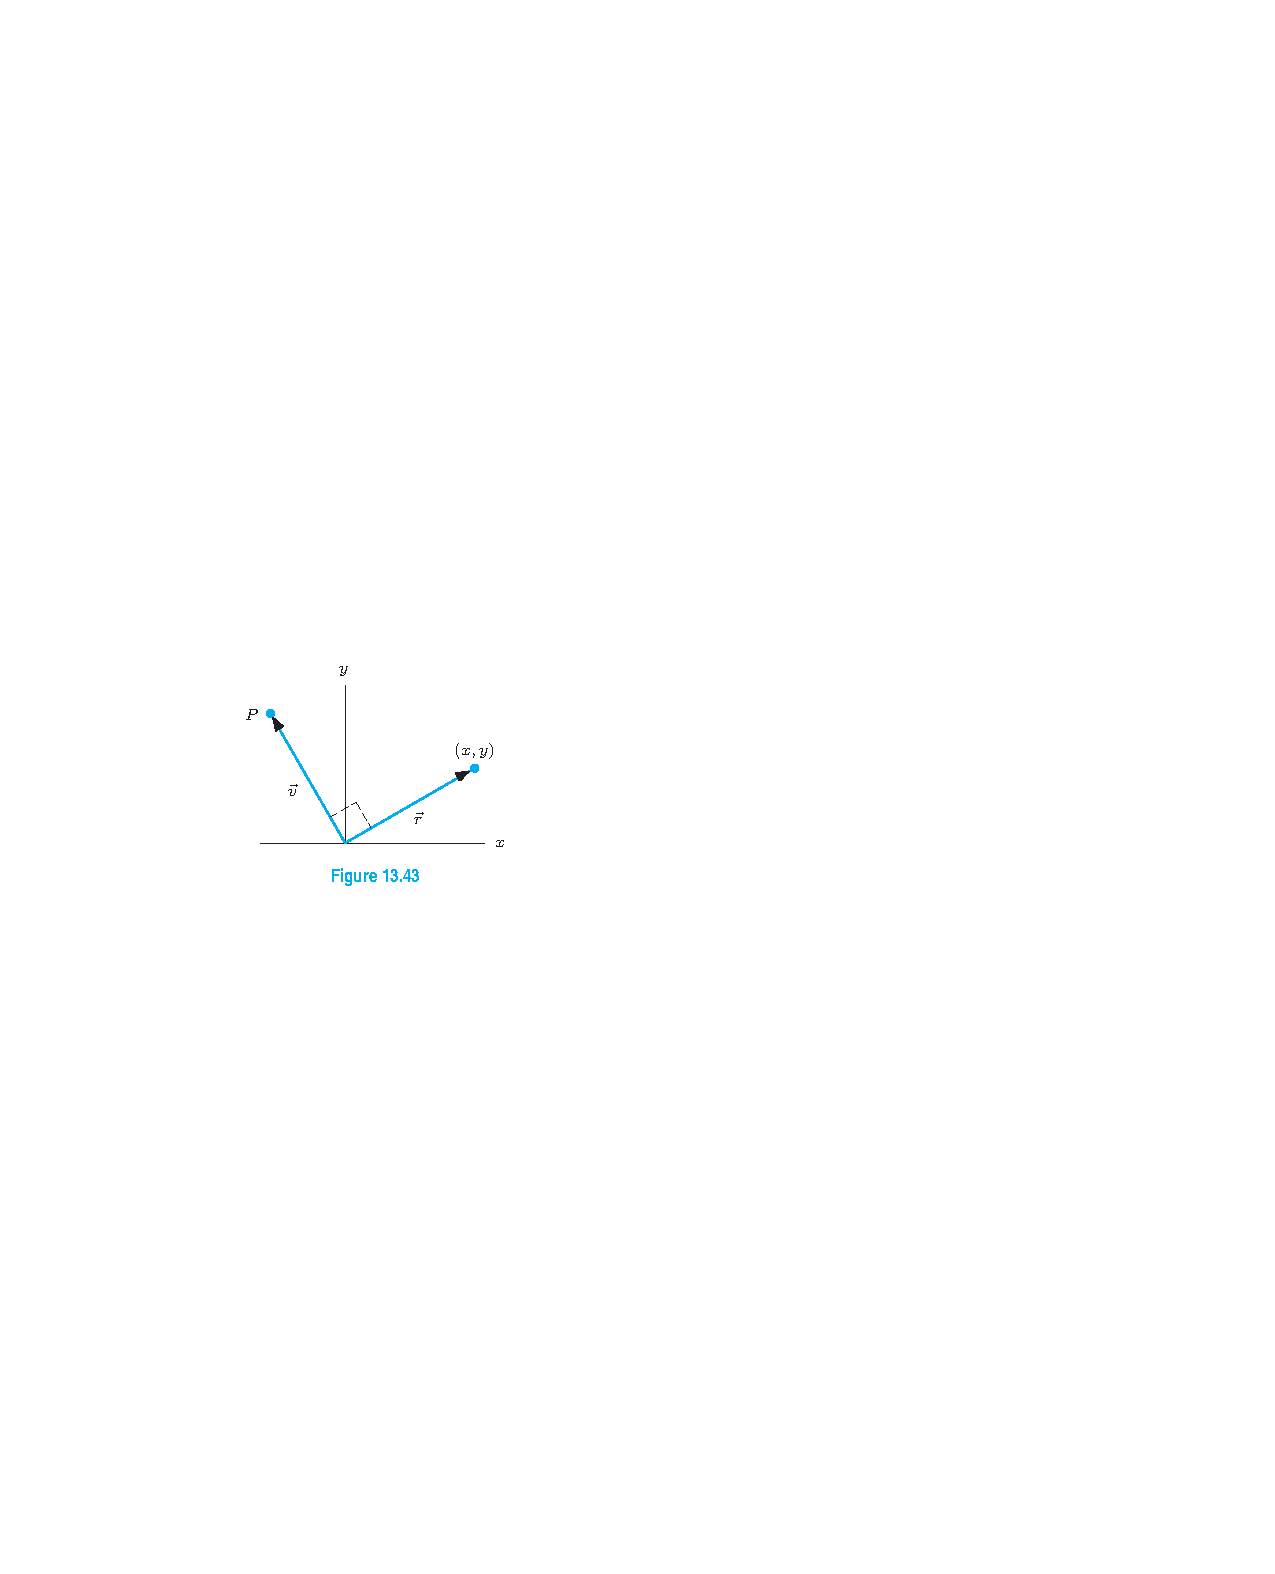
\includegraphics{img/HW04p2.pdf}

\begin{parts}
\item Use the geometric definition of the cross product to explain why $\mb{v} = \mb{k} \times \mb{r}$.
\begin{solution}
The cross product yields an area vector for the parallelogram bounded by $\vec k$ and $\vec r$.  In this picture, $\vec k$ is pointing out of the page, so is perpendicular to $\vec r$.  The magnitude of the vector is the area of the parallelogram.  The direction is normal to the parallelogram.  We have to use the right-hand-rule to determine which normal direction, though. Since $\vec{r}$ lies within the $xy$-plane, $\vec{k}$ is perpendicular to it and the parallelogram formed by $\vec{k}$ and $\vec{r}$ is a rectangle.  Its area should be $\Vert \vec{k}\Vert\Vert\vec{r}\Vert = \sqrt{x^2+y^2}$, so $\Vert \vec{k}\times\vec{r}\Vert = \sqrt{x^2+y^2}$.

For the direction, $\vec{v}$ is in the $xy$-plane so it is perpendicular to $\vec{k}$.  In addition, by construction it is perpendicular to $\vec{r}$.  The right hand rule has our palm align with $\vec{k}$, our fingers align with $\vec{r}$ and our thumb align with $\vec{v}$, so $\vec v$ is in the normal vector direction given by the right hand rule.  Since $\vec{v}$ is a rotation of $\vec{r}$ it has length $\sqrt{x^2+y^2}$.  We have that $\vec{v}$ is in the correct direction and has the correct length to be the area vector for the parallelogram given by $\vec{k}$ and $\vec{r}$ so $\vec{k}\times\vec{r} = \vec{v}$.

\end{solution}

\item Find the coordinates of $P$.  Explain your mathematical reasoning.
\begin{solution}
$P$ will have coordinates $(a,b,0)$ for some $a,b$ because it sits within the $xy$-plane.  We have that $\vec{v} \cdot\vec{r} = 0$ so $a x + by = 0$.  

In addition, $\sqrt{a^2+b^2} = \sqrt{x^2+y^2}$.

We have $ a= -b\frac{y}{x}$.  Substituting, we have $\sqrt{b^2\frac{y^2}{x^2}+b^2} = \sqrt{x^2+y^2}.$

Squaring both sides, this becomes $b^2(y^2/x^2+1) = x^2 + y^2$.

Pulling $x^2$ out of the denominator on the left hand side, this is $\frac{b^2}{x^2}(y^2+x^2) = (x^2+y^2)$ so
$b^2 = x^2$ and $b = \pm x$.

We can tell from the diagram that $b$ is positive when $x$ is positive, so $b = x$.  This implies that $a = -y$.

Trying $\vec{v} = -y\vec{i} + x\vec{j}$, it is clearly perpendicular to $\vec{r}$ and to $\vec{k}$, has the correct magnitude, and has the right-hand-rule direction that is desired. 
\end{solution}


\end{parts}

\item 
\begin{parts}
\item Find a vector $\mb{v}$ with all of the following properties: 
\begin{itemize}
\itemsep0em
\item Magnitude $20$, \item angle of $45^\circ$ with the positive $x$-axis, \item angle of $60^\circ$ with the positive $y$-axis, \item negative $z$-component.
\end{itemize}
\begin{solution}
Let $\mb v = v_1 \mb i + v_2 \mb j + v_3 \mb k.$

We have $\Vert \mb v \Vert = 20$.  

By equating the algebraic and geometric calculations of the dot product we will figure out the vector.

The vector forms an angle of $45^\circ$ with the $x$-axis, so $\ v \cdot \ i = \Vert \ v \Vert \cos \theta = 20 \cos \pi/4 = \frac{20}{\sqrt{2}}$.

$\ v \cdot \ i = v_1$ so $v_1 = 10\sqrt{2}$.

The vector forms an angle of $60^\circ$ with the $y$-axis so $\ v\cdot \ j = 20 \cos \pi/3 = 20\frac{1}{2} = 10.  \Rightarrow v_2 = 10.$

We have $\ v = 10\sqrt{2}\ i + 10\ j + v_3 \ k$ and $\sqrt{10^2(2) + 10^2 + v_3^2} = 20 \Rightarrow 300 + v_3^2 = 400$.  We have $v_3 = \pm \sqrt{100} = \pm 10$.  We are told that $v_3 < 0$ so the vector is

$\ v = 10(\sqrt{2}\ i + \ j - \ k)$.  

\end{solution}

\item A vector $\mb{v}$ of magnitude $v$ makes an angle $\alpha$ with the positive $x$-axis, $\beta$ with the positive $y$-axis and $\gamma$ with the positive $z$-axis.  Show that $\mb{v} = v\cos\alpha \mb{i} + v\cos\beta\mb{j} + v\cos\gamma\mb{k}$.  

\begin{solution}
We have $\vec v = v_1 \vec i + v_2 \vec j + v_3\vec k$.  

$\vec v \cdot \vec i = v_1 = \Vert \vec v \Vert \cos\alpha = v\cos\alpha$.

Similarly, we have $\vec v \cdot \vec j = v_2 = v\cos\beta$ and $\vec v \cdot \vec k = v_3 = v\cos\gamma$ so
$\vec v = v\cos\alpha \vec i + v\cos\beta \vec j + v\cos\gamma\vec k$.
\end{solution}


\item For angles $\alpha, \beta, \gamma$ as in $(b)$, show that $\cos^2\alpha+\cos^2\beta+\cos^2\gamma = 1$.

\begin{solution}
Consider $\vec v\cdot \vec v$.  This is $v_1^2+v_2^2+v_3^2 = v^2(\cos^2\alpha+\cos^2\beta+\cos^2\gamma)$ by the algebraic definition of the dot product.

In addition, $\vec v \cdot \vec v = \Vert \vec v \Vert^2 = v^2$.  We have \[v^2 = v^2(\cos^2\alpha+\cos^2\beta+\cos^2\gamma) \Rightarrow \cos^2\alpha+\cos^2\beta+\cos^2\gamma = 1.\]
\end{solution}


\end{parts}

\item We want to relate the area of a parallelogram to the area of its shadow in the $xy$-plane.



Consider a parallelogram $S$ lying in the plane $ z= mx + ny + c$.  It has a projection $R$ into the $xy$-plane.  Let $S$ be determined by the vectors $\mb{u} = u_1\mb{i}+u_2\mb{j}+u_3\mb{k}$ and $\mb{v} = v_1 \mb{i}+v_2\mb{j}+v_3\mb{k}$ as in the figure on the left below.  The figure on the right shows $S$ for a steeper plane.


\begin{center}
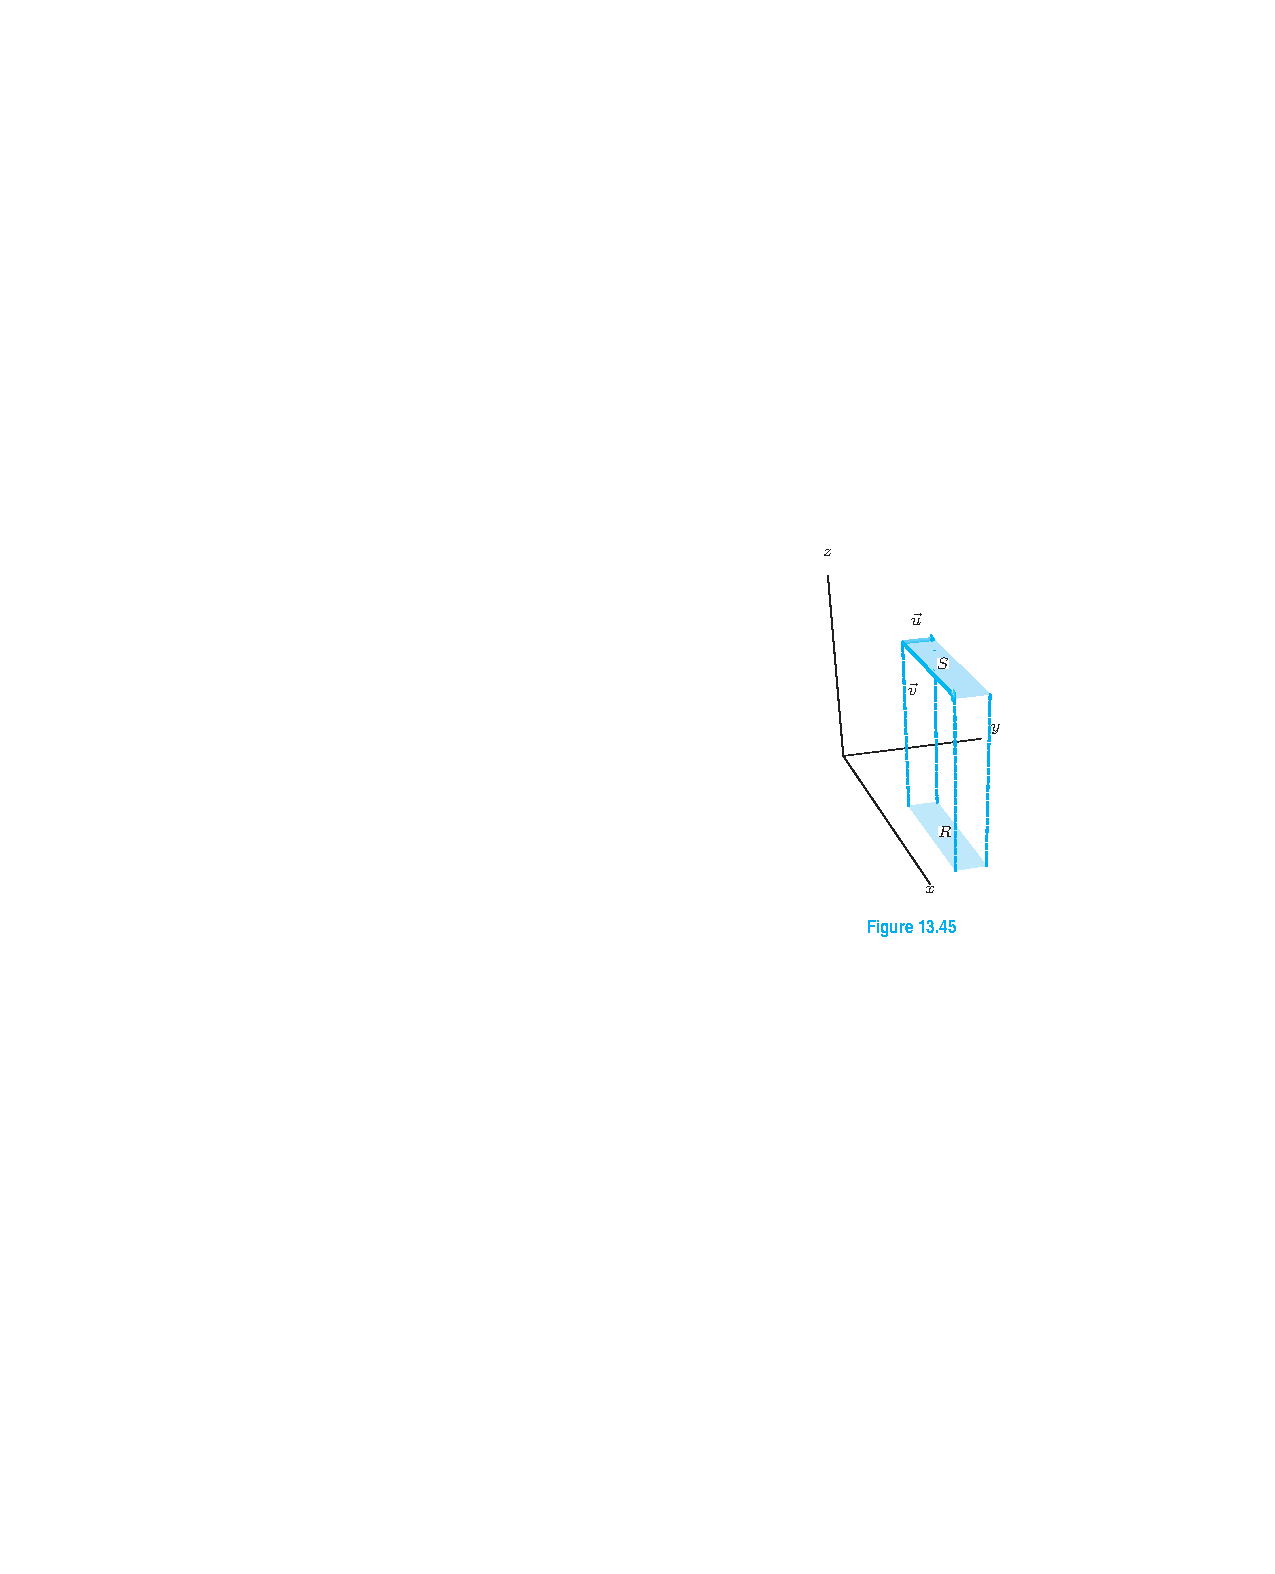
\includegraphics[height=3in]{img/HW04p1.pdf}\quad
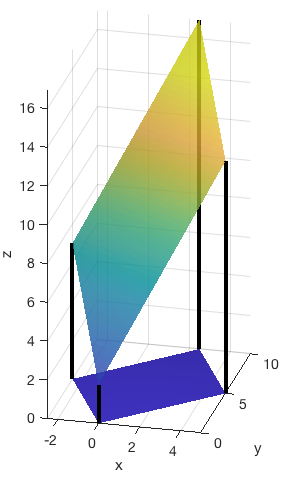
\includegraphics[height=3in]{img/pset03plane.png}
\end{center}



\begin{parts}
\item Use the matlab template for this problem set to produce three different plots of parallelograms and their projections into the $xy$-plane.  Insert the plots into your solution and submit the m-file with your code as a separate file when you submit your problem set.

Show your mathematical reasoning for the following:

\item Find the area of $R$. \emph{Find this in terms of $u_1, u_2, v_1, v_2$.}
\begin{solution}


$R$ is given by the projection of the parallelogram $S$.  $S$ is determined by vectors with $x$-, $y$-, and $z$-components.  $R$ should be determined by their shadows in the $xy$-plane, so the $z$-components are zero.  Thus $R$ is given by $\vec{u}_{proj} = \Delta x_1\vec{i} + \Delta y_1\vec{j}$ and $\vec{v}_{proj} = \Delta x_2\vec{i} + \Delta y_2\vec{k}$.

The area is given by length of the cross product.  The cross product is 
\begin{align*}
(\Delta x_1\vec{i}+\Delta y_1\vec{j})\times(\Delta x_2\vec{i}+\Delta y_2\vec{j}) &= \Delta x_1\vec{i} \times (\Delta x_2\vec{i}+\Delta y_2\vec{j})  + \Delta y_1\vec{j}\times(\Delta x_2\vec{i}+\Delta y_2\vec{j})  \\
&= \Delta x_1\Delta y_2\vec{i}\times\vec{j} + \Delta y_1\Delta x_2\vec{j}\times\vec{i} \\
&= (\Delta x_1\Delta y_2-\Delta y_1\Delta x_2)\vec{k},
\end{align*}
so its length is $\vert \Delta x_1\Delta y_2-\Delta y_1\Delta x_2\vert$.
\end{solution}

\item Find the area of $S$.  \emph{Find this in terms of the vector components}.
\begin{solution}
The area of $S$ is given by the length of the cross product of $\vec{u}$ and $\vec{v}$.  Using the formula for a general cross product, their cross product is \[\vec{u}\times\vec{v} = \vec{i}(\Delta y_1\Delta z_2 - \Delta z_1\Delta y_2) + \vec{j}(\Delta z_1\Delta x_2-\Delta x_1\Delta z_2) + \vec{k}(\Delta x_1\Delta y_2-\Delta y_1\Delta x_2).\]

Its length is 

$\sqrt{(\Delta y_1\Delta z_2 - \Delta z_1\Delta y_2)^2+(\Delta z_1\Delta x_2-\Delta x_1\Delta z_2)^2+(\Delta x_1\Delta y_2-\Delta y_1\Delta x_2)^2}$
\end{solution}

\item Show that \[\text{Area of }S = \sqrt{1+m^2+n^2}\cdot \text{ Area of }R.\]  %\emph{To show this mathematical fact, start with your expression for the left hand side from part (b).  Manipulate it in a series of steps until, after some number of steps, you have the expression on the right left hand side}.

%Notes for editing/hints: You know the direction of the normal vector, $\vec n$ (you can read it off of the plane equation).  So you know $\vec u \times \vec v$ is parallel to $\vec n$.  Can you write $\vec u \times \vec v$ as $c\vec n$ for some constant $C$?

\begin{solution}

\emph{one option:}

Let $A = \text{Area of }R = \vert \Delta x_1\Delta y_2-\Delta y_1\Delta x_2\vert$.  The area vector of $R$ is $A\vec k$.  The area vector of $S$ is  $\vec{i}(\Delta y_1\Delta z_2 - \Delta z_1\Delta y_2) + \vec{j}(\Delta z_1\Delta x_2-\Delta x_1\Delta z_2) + A\vec{k}.$

We know that the area vector of $S$ is parallel to $-m\vec i - n\vec j + \vec k$, the normal vector to the plane that $S$ lies within.  The constant of proportionality must be $A$ (by comparing the $\vec k$ components), so the area vector of $S$ $= A(-m \vec i -n \vec j + \vec k)$.

Finding the magnitude to compute the area of $S$ we have $\text{area of }S = A\sqrt{m^2+n^2+1}$, so the area of $S$ is equal to $\sqrt{m^2+n^2+1}\cdot\text{Area of }R$.



\emph{another option:}

We know that $S$ lies in the plane, so $\vec{v}$ and $\vec{u}$ are vectors in the plane.  We can think of $\Delta x_1$ as $\Delta x$, $\Delta y_1$ as $\Delta y$ and $\Delta z_1$ as $\Delta z$ for two points in the plane.  Using the equation of the plane, $\Delta z = m \Delta x + n\Delta y$ so $\Delta z_1 = m \Delta x_1+n\Delta y_1$.  Similarly, $\Delta z_2 = m\Delta x_2+n\Delta y_2$.

Substituting:
\begin{align*}
\text{Area of }S &= \sqrt{(\Delta y_1\Delta z_2 - \Delta z_1\Delta y_2)^2+(\Delta z_1\Delta x_2-\Delta x_1\Delta z_2)^2+(\Delta x_1\Delta y_2-\Delta y_1\Delta x_2)^2} \\
&= \sqrt{(\Delta y_1(m\Delta x_2+n\Delta y_2) - (m\Delta x_1+n\Delta y_1)\Delta y_2)^2+((m\Delta x_1+n\Delta y_1)\Delta x_2-\Delta x_1(m\Delta x_2+n\Delta y_2))^2+(\Delta x_1\Delta y_2-\Delta y_1\Delta x_2)^2} \\
&= \sqrt{(m\Delta y_1\Delta x_2+n\Delta y_1\Delta y_2 - m\Delta x_1\Delta y_2-n\Delta y_1\Delta y_2)^2+(m\Delta x_1\Delta x_2+n\Delta y_1\Delta x_2-m\Delta x_1\Delta x_2-n\Delta x_1\Delta y_2)^2+(\Delta x_1\Delta y_2-\Delta y_1\Delta x_2)^2} \\
&= \sqrt{(m\Delta y_1\Delta x_2 - m\Delta x_1\Delta y_2)^2+(n\Delta y_1\Delta x_2-n\Delta x_1\Delta y_2)^2+(\Delta x_1\Delta y_2-\Delta y_1\Delta x_2)^2} \\
&= \sqrt{m^2(\Delta y_1\Delta x_2 - \Delta x_1\Delta y_2)^2+n^2(\Delta y_1\Delta x_2-\Delta x_1\Delta y_2)^2+(\Delta x_1\Delta y_2-\Delta y_1\Delta x_2)^2} \\
&= \sqrt{m^2+n^2+1}\sqrt{(\Delta x_1\Delta y_2-\Delta y_1\Delta x_2)^2} \\
&= \sqrt{m^2+n^2+1}\cdot\text{Area of }R
\end{align*}

This tells us that as the plane slants the area of $S$ becomes a larger multiple of the area of $R$.  The minimum area occurs when $m = n = 0$, so for a flat plane parallel to the $xy$-plane.  In that case the two areas are equal.



\end{solution}
\item Show that the area of the projection of $S$ into the $xy$-plane is $\vert\mb A \cdot \mb k\vert$ where $\mb A$ is the area vector for $S$.  Write a similar expression that you think would give the area of the projection of $S$ into the $xz$-plane.
\begin{solution}

We found above that $\mb A$, the area vector for $S$, has $\mb k$ component $A\mb k$ where $A$ is the area of $R$.  Since $\mb A \cdot \mb k = A$, this projection is the area of $R$.

Presumable $\vert \vec A \cdot \vec j \vert$ would give the area of the projection of $S$ into the $xz$-plane, since $\vec j$ is the normal to the $xz$-plane (just as $\vec k$ was the normal to the $xy$-plane).
\end{solution}
\end{parts}


% \emph{The idea in this problem is going to underpin our ability to work with surfaces later in the course.  To set up surface integrals, we will often want to cut a surface into parallelograms.  We will need to be able to relate the area of each parallelogram to the area of its projection into the $xy$-plane.}

% If you get stuck think about a lower dimensional version of the problem:
% \begin{itemize}
%     \item Consider the $2$-space version of this.  You have a line segment $L$ along the line $ y = mx + b.$  Let $L$ be determined by the vector $\vec u = \Delta x\vec i + \Delta y\vec j.$  Let $D$ be the length of the projection of $L$ onto the $x$-axis.  Show that $\text{Length of }L = \sqrt{1+m^2}\cdot \text{ Length of }D.$  Translate the way you treated $\Delta y$ in this problem to how you can treat $\Delta z_1$ and $\Delta z_2$ in the parallelogram problem.
% \end{itemize}


% For reference, problems are identified as: 

% Hughes-Hallett 12.1 2, 5, 7, 7, 13, 28, 29, 30, 31, 12.2 15, 16

% Stewart 13.1 3, 14.1 1

\question (Revisiting land lost to sea level change).  Last week you approximated the land area lost to sea level rise in an image that included Massachusetts.
\begin{parts}
\part After discussing the problem with your classmates, choose two different approximation schemes that you'll use to redo the calculation this week.  Implement each method yourself.  \emph{You may choose the method you used last week, as well as a different method of approximating}.
\part Use each of these methods on
\begin{itemize}
    \item the cropped image with no smoothing and no downsampling
    \item the cropped image with a little smoothing and a little downsampling
    \item the cropped image with more smoothing and a little downsampling
    \item the cropped image with a little smoothing and more downsampling
    \item the cropped image with more smoothing and more downsampling
\end{itemize}
to produce ten different estimates of the land area lost (measure the land area in km$^2$).
\part Plot your ten estimates.  \emph{Insert the plot into your problem set write-up and remember to add labels to the axes.} Given these ten (presumably different) estimates, provide a single estimate for the approximate land lost and explain how you chose that estimate.
\end{parts}


\question (cosine similarity) The following time series data is course enrollment data for four courses at Harvard:

\begin{tabular}{| c | c|c|c|c|c|c|}
\hline
course & 2009 & 2010 & 2011 & 2012 & 2013 & 2014 \\
\hline
\hline
cs50 &337 &478 &607&715&693&825\\
stat 110 & 216&258&272&308&454&321 \\
multi & 620&568&649&690&767&777 \\
greek hero & 95&68&219&221&236&40 \\
\hline
\end{tabular}

\emph{The `multi' column aggregates all multivariable courses taught at Harvard in that year}

These vectors are in 6-dimensional space.
\begin{parts}
\item Use the cosine of the angle between the vectors as a measure of their similarity.  This is the \textbf{cosine similarity}.  Edit the Matlab code provided to compute the cosine similarity between each pair of vectors.

According to this measure, 
\begin{itemize}
    \item which two course enrollment time-series are most similar?
    \item which two are least similar?
    \item how wide is the variation?
\end{itemize}

\item Instead of directly comparing the values in the time series, it is common to compare the variation of each time-series from its own mean.  This is called \textbf{centering} the data.  Use centered data to answer the questions above.  \emph{Add code for this to the end of your matlab file.}

\item The cosine similarity of centered data is also referred to as the \textbf{correlation coefficient} of the two data vectors.  Describe, in words, the relationship between the data in two vectors when the correlation coefficient is
\begin{itemize}
    \item near $1$
    \item near $0$
    \item near $-1$
\end{itemize}
\end{parts}

\end{questions}


Late work policy:  Because of the unusual circumstances of our semester, all students have access to deadline flexibility when needed.  You may assume that extensions of up to two days will be approved without issue.  Request those via direct message on Slack.  When you request an extension, specify your preferred new deadline for the assignment.

Late WeBWorK is difficult to arrange (it requires a manual override of the course settings), so I suggest planning ahead to complete it on time.
\vspace{1cm} 
\hrule
\vspace{1cm}

\end{document}